%%%% PROPOSED MODELS %%%%
\chapter{Auditory models for evaluating navigational methods}\label{chap:05_Proposed_Models}
In this chapter, we propose and validate models that predict perceived source localization (i.e., the direction of a source relative to the listener) and spectral coloration (changes in the spectral content of a sound) for the specific purpose of evaluating navigational methods for ambisonics-encoded sound fields.
Previous evaluations of navigational methods have typically relied on binaural localization models, which conflate the effects of the navigational method with those of the adopted ambisonics-to-binaural rendering approach, and previous studies on navigation-induced coloration have been largely qualitative.
Consequently, in this chapter, we seek to develop perceptually-relevant auditory models that can be applied directly to translated ambisonics impulse responses (i.e., before rendering to binaural) and give numerical predictions for localization direction and coloration.

\section{Introduction}\label{sec:05_Proposed_Models:Introduction}
Of the several navigational methods reviewed in \chapref{chap:03_Navigation_Techniques}, we expect that they all may degrade localization information and induce spectral coloration, leading to errors in the perceived directions of sound sources and audible changes in the spectral content of the signals, respectively.
The severity of such penalties needs to be investigated and quantified in order to both compare existing navigational methods and develop novel ones.
Although subjective testing is the most direct method of evaluating and comparing navigational methods, such tests are often lengthy and costly, which motivates the use of objective metrics that enable quick assessments of navigational methods.

% Review of previous work focusing on the remaining problems (questions or deficiencies) the present paper claims to contribute to solving
\subsection{Previous work and remaining problems}
Several recent studies have investigated the localization accuracy of various navigational methods.
\citet{Winter2014} evaluated the localization accuracy of the plane-wave-based translation method of \citet{SchultzSpors2013} (reviewed in \secref{sec:03_Navigation_Techniques:PW_Technique}) using the binaural localization model of \citet{Dietz2011} (reviewed in \secref{sec:04_Auditory_Models:Binaural_Localization_Model}) to predict perceived localization.
\citet{TylkaChoueiri2015} compared the localization errors incurred by three extrapolation-based translation methods (reviewed in \secref{sec:03_Navigation_Techniques:Extrapolation_Methods}) using the velocity and energy localization vectors developed by \citet{Gerzon1992} (reviewed in \secref{sec:04_Auditory_Models:Localization_Vectors}).
However, this analysis neglected the precedence effect, which is expected to play an important role in the context of sound field navigation, as an accurate virtual translation of the listener necessarily involves direction-dependent time shifting of incident signals.
Consequently, more recently, \citet{TylkaChoueiri2016} evaluated the localization accuracy of their proposed interpolation-based navigational method (introduced here in \chapref{chap:08_Proposed_Method}) using an extension of a precedence-effect-based localization vector developed by \citet{Stitt2016} (reviewed in \secref{sec:04_Auditory_Models:PE_Energy_Vector}), which was itself an extension of Gerzon's original energy vector.
Although the model of \citeauthor{Stitt2016} has been validated through listening tests and shows improvements compared to binaural localization models (specifically, those by \citet{Dietz2011} and \citet{Lindemann1986a}) the more recent extension by \citet{TylkaChoueiri2016} had not, at the time of publication, been validated through listening tests.

Additionally, recent studies have investigated spectral colorations induced by various navigational methods.
\citet{HahnSpors2015b} evaluated spectral coloration induced by the plane-wave translation method \citep{SchultzSpors2013} by visually examining impulse and frequency responses.
In a similar manner, \citet{TylkaChoueiri2016} evaluated and compared the spectral coloration induced by both their proposed interpolation method and the linear interpolation method of \citet{Southern2009} (reviewed in \secref{sec:03_Navigation_Techniques:XF_Technique}).
While it is clear from these studies that most (if not all) existing navigational methods tend to induce at least some spectral coloration, both analyses were largely qualitative.
Consequently, it remains difficult to compare these colorations between methods without numerical measures of perceptible coloration.

% A statement of the paper's main question(s) and goal(s), followed by a succinct description of the general method and approach to be described in the paper
\subsection{Objectives and approach}
In this chapter, we present models for perceived source localization and spectral coloration which we have developed for the purpose of evaluating and comparing methods for virtual navigation of ambisonics-encoded sound fields.
In order to isolate any errors introduced by the navigational method under test (which operates in the ambisonics domain) from those introduced through rendering to binaural, we developed models that are independent of any choice of ambisonics-to-binaural rendering approach (several of which are reviewed in \secref{sec:02_Acoustical_Theory:Binaural_Rendering}) since they operate directly on ambisonics impulse responses.
In contrast, although not explicitly investigated here, we expect the predictions of binaural models to be sensitive to the choice of binaural rendering approach and/or to the choice of head-related transfer function (HRTF).

For these models to be of any practical use, they must also be perceptually relevant, in that the predictions of the models should agree with subjective listening test responses.
Consequently, we conducted two listening experiments (one each for localization and coloration), the results of which were used to determine parameters of the proposed models.
We then validated the proposed models through comparisons against alternative models in terms of their agreement with the experimental data.

% A brief section by section description of the structure of the paper
In \secreftwo{sec:05_Proposed_Models:Localization_Model}{sec:05_Proposed_Models:Coloration_Models}, we describe the proposed localization and coloration models, respectively.
Then, in \secref{sec:05_Proposed_Models:Listening_Tests}, we describe the listening experiments conducted to validate the proposed models.
In \secref{sec:05_Proposed_Models:Results}, we compare the results of the listening experiments with predictions of the models, and finally, in \secref{sec:05_Proposed_Models:Conclusions}, we draw conclusions based on these results.

%%%% Auditory Models %%%%
%% Proposed Localization Model
\section{Localization model}\label{sec:05_Proposed_Models:Localization_Model}
Recently, \citet{Stitt2016} proposed an extension to incorporate the precedence effect into the energy vector of \citet{Gerzon1992}.
In their paper, \citeauthor{Stitt2016} also showed that their proposed model achieves improved localization prediction accuracy compared to the binaural models of \citet{Dietz2011} and \citet{Lindemann1986a}.
Motivated by these results, we proposed in a recent paper \citep{TylkaChoueiri2016} an extension to this localization model; here, we describe and revise our proposed extension.

We begin by converting the ambisonics impulse response into a set of $Q$ impulse responses for a specified grid of plane-wave directions, $\hat{v}_q$, with $q \in [1,Q]$.
For ambisonics order $L$, there are $N = (L + 1)^2$ ambisonics signals, $a_n(t)$, with $n \in [0, N-1]$, and the corresponding plane-wave signals, $\mu$, are given by \eqnref{eq:02_Acoustical_Theory:A2mu}.%
\footnote{Alternatively, this plane-wave decomposition could be computed using a pseudoinversion approach, as described in \eqnref{eq:02_Acoustical_Theory:A2mu_Pinv}, or a compressed sensing approach, as described by \citet[Eq.~(10)]{Epain2009}.}
The grids of directions (also called ``nodes'') used here are given by \citet{FliegeMaier1999}; these grids and their corresponding quadrature weights are freely available online.\citefooturl{FliegeNodesURL}
As this discrete plane-wave sound field would generally be rendered via quadrature integration (see \eqnref{eq:02_Acoustical_Theory:PW_Quadrature_Rendered_Field}), the impulse response for each plane-wave term is given by $g_q(t) = w_q \mu(t,\hat{v}_q)$, where $w_q$ is the quadrature weight for the direction $\hat{v}_q$.

Next, we identify and isolate temporally-distinct impulse response ``wavelets.''
To do this, we apply a $4^\textrm{th}$-order Butterworth high-pass filter with a cut-off frequency of 500~Hz to all impulse responses in the set and compute the global maximum (i.e., the largest absolute value over all impulse responses in the set).
For each impulse response, we take the absolute value and identify any peaks (i.e., local maxima) whose amplitudes are at least $G_\text{min}$~dB relative to the global maximum ($G_\text{min} \leq 0$~dB).
If no such peaks exist in a given impulse response, then that response in its entirety is treated as a wavelet.
If at least one such peak exists, then, around each peak, we apply a Tukey window beginning $\tau_\text{w}$~ms before the peak and ending either $\tau_\text{w}$~ms after the peak, or at the position of the following peak, whichever yields a larger window length.
Both the cosine fade-in and fade-out of the Tukey window are $\tau_\text{w}$~ms in duration.
In this way, a single impulse response may be split into several wavelets.%
\footnote{A simpler implementation of this stage of the model might follow a more traditional, uniformly-partitioned STFT approach, but we do not explore this idea here.}
For each wavelet, we apply a 10\% ($-20$~dB, now relative to the peak of that particular wavelet) threshold to determine the time-delay of the onset.

For the purposes of this model, we consider each wavelet to be a distinct sound source, such that wavelets extracted from the same impulse response originate from the same direction, but arrive at different times, given by their onset times.
Taking the Fourier transform of each wavelet yields complex-valued, frequency-dependent gains, $G_{q'}$, of the $q'{}^\text{th}$ wavelet, where $q' \in [1,Q']$ and $Q' \geq Q$ is the total number of wavelets.
We then average these gains in critical bands using a gammatone filter bank (see \figref{fig:04_Auditory_Models:Gammatone_Filters}),
such that the frequency-averaged gains are given by
\begin{equation}\label{eq:05_Proposed_Models:Localization_Model:FreqAvg_Gain}
\overline{G}_{q'}(f_c) = \frac{\displaystyle \int_{-\infty}^\infty |H_\Gamma(f;f_c)| |G_{q'}(f)| df}{\displaystyle \int_{-\infty}^\infty |H_\Gamma(f;f_c)| df},
\end{equation}
where the gammatone filters are taken for a set of ERB-spaced center frequencies spanning the range $f \in [20~\text{Hz}, 20~\text{kHz}]$.

For each frequency band, we feed these gains into the model, yielding a frequency-dependent predicted localization vector $\vec{\nu}_\textrm{PE}(f_c)$, given by
\begin{equation}\label{eq:05_Proposed_Models:PE_Energy_Vector}
\vec{\nu}_{\textrm{PE}}(f_c) = \frac{ \sum_{q'} |w_{q'}(\alpha) \overline{G}_{q'}(f_c)|^2 \, \hat{v}_{q'}}{ \sum_{q'} |w_{q'}(\alpha) \overline{G}_{q'}(f_c)|^2},
\end{equation}
where $\alpha$ is a parameter of the original model of \citet{Stitt2016} (discussed in \secref{sec:04_Auditory_Models:PE_Energy_Vector}) and $w_{q'}(\alpha)$ is a perceptual weight (based on the precedence-effect) for the $q'{}^\text{th}$ wavelet.
Similarly, we define a perceptually-weighted velocity vector, given by
\begin{equation}\label{eq:PE_Velocity_Vector}
\vec{\nu}_{\textrm{PV}}(f_c) = \text{Re} \left[ \frac{ \sum_{q'} w_{q'}(\alpha) \overline{G}_{q'}(f_c) \, \hat{v}_{q'}}{ \sum_{q'} w_{q'}(\alpha) \overline{G}_{q'}(f_c)} \right],
\end{equation}
where $\text{Re}(\cdot)$ denotes taking the real part of the argument.
Note that we include this step of ``taking the real part'' in our definition only to maintain consistency with the original definition of the velocity vector, given by \citet[section 4]{Gerzon1992}, in which complex-valued gains are used (see \eqnref{eq:04_Auditory_Models:Velocity_Vector}).
However, in our case, all $\overline{G}_{q'}$ are already real-valued (see \eqnref{eq:05_Proposed_Models:Localization_Model:FreqAvg_Gain}), so taking the real part has no effect on the result.
This deviation from the original definition may be justified since the time-dependence of the sources is now captured in the precedence-effect-based weights, so each source's phase is no longer needed.

We then combine the velocity vector below 700~Hz and the energy vector above into a single, frequency-dependent vector, given by
\begin{equation}
\vec{\nu}_{\textrm{PC}}(f_c) =
\begin{cases}
\displaystyle \frac{\left\| \vec{\nu}_{\textrm{PE}}(f_\text{XO}) \right\|}{\left\| \vec{\nu}_{\textrm{PV}}(f_\text{XO}) \right\|} \cdot \vec{\nu}_{\textrm{PV}}(f_c), & \text{for}~f_c \leq f_\text{XO}, \\
\vec{\nu}_{\textrm{PE}}(f_c), & \text{for}~f_c > f_\text{XO},
\end{cases}
\end{equation}
where $\|\cdot\|$ denotes the $\ell^2$ norm (Euclidean distance) of a vector, $f_\text{XO}$ is the ``crossover'' frequency, equal to the center frequency nearest to 700~Hz, and we have introduced a normalization factor to match low- and high-frequency vector magnitudes.
Finally, we compute a weighted-average vector, which depends on the stimulus signal and is given by
\begin{equation}
\vec{\nu}_{\textrm{P}} = \frac{\sum_c \overline{X}(f_c)\, \vec{\nu}_{\textrm{PC}}(f_c)}{\sum_c \overline{X}(f_c)},
\end{equation}
where the weights $\overline{X}(f_c)$ are the stimulus signal's energy in each critical band, given by
\begin{equation}
\overline{X}(f_c) = \frac{\displaystyle \int_{-\infty}^\infty |H_\Gamma(f;f_c)| |X(f)|^2 df}{\displaystyle \int_{-\infty}^\infty |H_\Gamma(f;f_c)| df},
\end{equation}
and $X(f)$ is the Fourier transform of the stimulus signal.

In addition to the three free model parameters ($Q$, $\tau_\text{w}$, and $G_\text{min}$) defined above, the original model of \citet{Stitt2016} retains one free parameter, $\alpha \in [0,1]$, which specifies the relative importance of stationary (i.e., time-averaged) to transient information in the stimulus signal (see \secref{sec:04_Auditory_Models:PE_Energy_Vector}).
As will be described below in \secref{sec:05_Proposed_Models:Localization_Results}, we determined optimal values for these four parameters based on a best fit of the model's predictions to the data from the listening experiment.

%% Proposed Coloration Models
\section{Coloration models}\label{sec:05_Proposed_Models:Coloration_Models}
In this work, we followed the approach of \citet{Wittek2007} and developed linear regression models to predict subjective ratings of coloration given some combination of the coloration metrics reviewed in \secref{sec:04_Auditory_Models:Coloration_Metrics}.
As discussed in \chapref{chap:04_Auditory_Models}, we define each of these metrics \textit{relative} to some reference signal.
Consequently, each metric is computed using both a \textit{test sample} (i.e., the ambisonics impulse response for the listening position after processing through some navigational method) and a \textit{reference sample} (i.e., the ambisonics impulse response captured directly at the listening position).

In this work, we used the combinations of coloration metrics listed in \tabref{tab:Coloration_Models} to create multiple linear regression models, each of which predicts subjective ratings of coloration.
Regression coefficients were found by fitting the predictions of each model to the data, as will be discussed below in \secref{sec:05_Proposed_Models:Coloration_Results}.

% Table of coloration models and corresponding metrics
\begin{table}[t]
\centering
 \begin{tabular}{|c|c|} \hline
 \textbf{Model Name} & \textbf{Metrics Used} \\ \hline
 Proposed & $\rho_\eta, \sigma_\eta, E_\text{pk}, E_\text{n}$ \\
 \citet{Kates1984} & $\rho_{e_\text{CS}}, \sigma_{e_\text{CS}}$ \\
 \citet{Pulkki1999} & $\rho_{e_\text{CLL}}, \sigma_{e_\text{CLL}}$ \\
 \citet{Wittek2007} & $\rho_{e_\text{IS}}, \sigma_{e_\text{IS}}$ \\ \hline
 \end{tabular}
 \caption{Metrics used for each coloration model.}
 \label{tab:Coloration_Models}
\end{table}

%%%% Validation of Proposed Models %%%%
\section{Listening experiments}\label{sec:05_Proposed_Models:Listening_Tests}
Two listening experiments were conducted in an acoustically-treated listening room,
where the listener was seated and given a pair of headphones.
Four subjects, all male, ages 25--30 years, participated in the experiments;
each subject is an experienced audio engineer or researcher.
Prior to the experiments, each subject's HRTFs were measured in an anechoic chamber.
These HRTFs were measured also as part of an ongoing project to compile a database of measured HRTFs \citep{Sridhar2017}.
The procedures employed to collect and process these measurements are reproduced in \apxref{chap:A4_HRTF_Measurements}.

Each subject's HRTFs were used to generate an individualized ambisonics-to-binaural rendering configuration for the ambiX binaural decoder plug-in \citep{Kronlachner2013,ambiXPlugInURL}.
In this decoder, we performed a basic (pseudoinverse) ambisonic decoding (see \eqnref{eq:02_Acoustical_Theory:PinvDecoder}) for a 36-node Fliege grid and filtered each virtual loudspeaker's signal by the nearest measured HRTF.
This decoder was generated using an early version of the SOFA/ambiX binaural rendering (SABRE) toolkit, which was developed by the present author and is described in \apxref{chap:A2_SABRE_Toolkit}.
The headphones (Stax SR-009) were equalized for each subject using a regularized, least-squares equalization filter \citep{ScharerLindau2009}.

The test samples were produced using the weighted average method and a regularized least-squares interpolation method (described in \secreftwo{sec:03_Navigation_Techniques:XF_Technique}{sec:08_Proposed_Method:Reg-LS_Technique}, respectively), employed for microphone spacings of 10, 30, or 50~cm.
The test samples were rendered from 4\textsuperscript{th}-order ambisonics room impulse responses for microphone positions distributed on both sides of the listening position, as illustrated by the empty circles in \figref{fig:Test_Geometry}.
For the localization test, these impulse responses were measured with a 32-capsule spherical microphone array, using phase-controlled exponential sine sweeps and an exact deconvolution of the recorded signals by the input signal, as described in \apxref{chap:A5_Impulse_Response}.
For the coloration test, on the other hand, the impulse responses were simulated using a MATLAB-based room acoustics simulator%
\footnote{In this work, we used the Multichannel Room Acoustics Simulator (\textsc{MCRoomSim}) package \citep{Wabnitz2010,MCRoomSimURL}.}
with a room model similar in size and acoustics to the actual listening room.
Also included in each test were reference samples, measured at the listening position and for which no interpolation was performed.
All stimuli were presented at levels between 60~dB and 78~dB (A-weighted), $\pm4$~dB.

% Diagram of source/mic positions
\begin{figure}[t]
\centering
  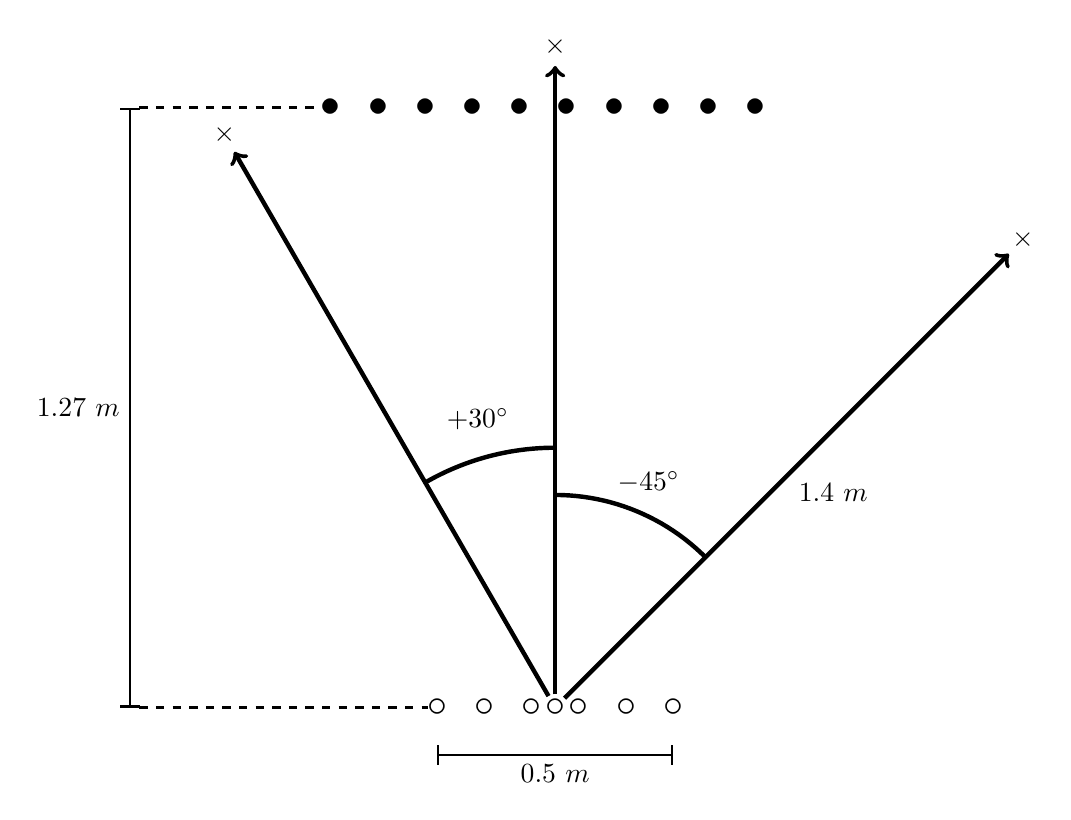
\begin{tikzpicture}[scale=6]
% Parameters
\def\radius{1.4};
\def\arrowStart{0.02};
\def\arrowScale{0.97};
\def\arcRadius{0.5};
\def\micSpacing{0.1};
\def\spkrSpacing{0.05};
\def\spkrDistance{1.27};
\def\offset{0.02};
\pgfmathsetmacro\colLefty{cos(-30)*\radius}
\pgfmathsetmacro\colLeftx{sin(-30)*\radius}
\pgfmathsetmacro\colCentery{cos(0)*\radius}
\pgfmathsetmacro\colCenterx{sin(0)*\radius}
\pgfmathsetmacro\colRighty{cos(45)*\radius}
\pgfmathsetmacro\colRightx{sin(45)*\radius}
\pgfmathsetmacro\arcLefty{cos(-15)*1.1*\arcRadius}
\pgfmathsetmacro\arcLeftx{sin(-15)*1.1*\arcRadius}
\pgfmathsetmacro\arcRighty{cos(22.5)*0.9*\arcRadius}
\pgfmathsetmacro\arcRightx{sin(22.5)*0.9*\arcRadius}

% Arrows
\draw[ultra thick,->] ({\arrowStart*\colLeftx},{\arrowStart*\colLefty}) -- (\arrowScale*\colLeftx,\arrowScale*\colLefty);
\draw[ultra thick,->] ({\arrowStart*\colCenterx},{\arrowStart*\colCentery}) -- (\arrowScale*\colCenterx,\arrowScale*\colCentery);
\draw[ultra thick,->] ({\arrowStart*\colRightx},{\arrowStart*\colRighty}) -- (\arrowScale*\colRightx,\arrowScale*\colRighty);
\node[below right] at (0.5*\colRightx,0.5*\colRighty){$1.4~\text{m}$};
\node at (\colLeftx,\colLefty){$\times$};
\node at (\colCenterx,\colCentery){$\times$};
\node at (\colRightx,\colRighty){$\times$};

% Distances
\draw[thick,|-|] (-2.5*\micSpacing,-0.1) -- (2.5*\micSpacing,-0.1) node[below, pos=0.5]{$0.5~\text{m}$};
\draw[thick,|-|] (-0.9,0) -- (-0.9,\spkrDistance) node[left, pos=0.5]{$1.27~\text{m}$};
\draw[thick, dashed] (-0.9+\offset,\spkrDistance) -- (-9.5*\spkrSpacing-\offset,\spkrDistance);
\draw[thick, dashed] (-0.9+\offset,0) -- (-2.5*\micSpacing-\offset,0);

% Arcs
\draw[ultra thick,domain=45:90] plot ({0.9*\arcRadius*cos(\x)}, {0.9*\arcRadius*sin(\x)});
\draw[ultra thick,domain=90:120] plot ({1.1*\arcRadius*cos(\x)}, {1.1*\arcRadius*sin(\x)});
\node at (1.15*\arcLeftx,1.15*\arcLefty){$+30^\circ$};
\node at (1.15*\arcRightx,1.15*\arcRighty){$-45^\circ$};

% Mic positions
\node at (-2.5*\micSpacing,0){\Large $\circ$};
\node at (-1.5*\micSpacing,0){\Large $\circ$};
\node at (-0.5*\micSpacing,0){\Large $\circ$};
\node at (0*\micSpacing,0){\Large $\circ$};
\node at (0.5*\micSpacing,0){\Large $\circ$};
\node at (1.5*\micSpacing,0){\Large $\circ$};
\node at (2.5*\micSpacing,0){\Large $\circ$};

% Speaker positions
\node at (-9.5*\spkrSpacing,\spkrDistance){\Large $\bullet$};
\node at (-7.5*\spkrSpacing,\spkrDistance){\Large $\bullet$};
\node at (-5.5*\spkrSpacing,\spkrDistance){\Large $\bullet$};
\node at (-3.5*\spkrSpacing,\spkrDistance){\Large $\bullet$};
\node at (-1.5*\spkrSpacing,\spkrDistance){\Large $\bullet$};
\node at (0.5*\spkrSpacing,\spkrDistance){\Large $\bullet$};
\node at (2.5*\spkrSpacing,\spkrDistance){\Large $\bullet$};
\node at (4.5*\spkrSpacing,\spkrDistance){\Large $\bullet$};
\node at (6.5*\spkrSpacing,\spkrDistance){\Large $\bullet$};
\node at (8.5*\spkrSpacing,\spkrDistance){\Large $\bullet$};
\end{tikzpicture}
  \caption[Diagram of microphone and source positions used in the listening tests.]{
  Diagram of microphone and source positions used in the listening tests.
  The empty circles indicate the microphone positions,
  the filled circles indicate the source positions used in the localization test, and
  the crosses indicate the source positions used in the coloration test.}
  \label{fig:Test_Geometry}
\end{figure}

\subsection{Localization test}\label{sec:05_Proposed_Models:Localization_Test}
To measure perceived source localization, we conducted a virtual source localization test, in which the listener was seated approximately $1.27$~m in front of a horizontal linear array of 30 transducers spaced 5~cm apart (note that the array served only as a visual reference to promote an externalized perception of the sound by the listener).
An infrared head-tracking device (NaturalPoint TrackIR) was used to maintain a stationary sound field as the subject's head rotated.
The test consisted of 1 training round followed by 5 rounds of testing, with optional short breaks in between each round for the subject to stand up and take off the headphones.
In each round, the subject was presented with 14 randomly-selected samples (2 references and 12 test samples in each round), all of which were a short ($\sim2$~second) clip of male English speech.
The graphical user interface (GUI) presented to the subject is shown in \figref{fig:05_Proposed_Models:Localization_GUI} and the sheet of instructions provided to the subject is shown in \figref{fig:05_Proposed_Models:Localization_Instructions} (at the end of this chapter).
The intended source directions produced in the test corresponded to 10 of the 30 transducers, spanning approximately $\pm20^\circ$ azimuth on the horizontal plane, as illustrated by the filled circles in \figref{fig:Test_Geometry}.
The subject was asked to identify the direction from which the sound appeared to originate, and subsequently face it.
The subject's head-angle (obtained from the head-tracking device) was then captured and recorded as the perceived direction of the source.
The subject was able to repeat each sample any number of times until confident about the location of the source.

\begin{figure}[t]
  \centering
  \setlength{\fboxsep}{0pt}
  \setlength{\fboxrule}{1pt}
  \fbox{\includegraphics[width=0.58\textwidth]{05_proposed_models/figures/LocalizationTestGUI}}
  \caption{Screenshot of the GUI for the localization test.}
  \label{fig:05_Proposed_Models:Localization_GUI}
\end{figure}

\subsection{Coloration test}\label{sec:05_Proposed_Models:Coloration_Test}
To collect subjective ratings of coloration, we conducted an \citet{ITU-R-BS.1534-3} MUSHRA (MUltiple Stimuli with Hidden Reference and Anchor) test,
administered in the same listening room and with the same headphones, but without head-tracking.%
\footnote{The loudspeaker array which served as a visual reference for the localization test was still present for this test, but the subjects were informed that it no longer corresponded to the signals they would be hearing.}
The test consisted of 1 training round followed by 3 rounds of testing, with optional short breaks between rounds.
In each round, the subject was presented with 9 ``test samples'' (actually 6 test samples, 2 anchors, and a hidden reference) and a labeled reference sample, all of which were a short ($\sim3$~second) clip of pink noise.
The GUI presented to the subject is shown in \figref{fig:05_Proposed_Models:Coloration_GUI} and the sheet of instructions provided to the subject is shown in \figref{fig:05_Proposed_Models:Coloration_Instructions} (at the end of this chapter).
The so-called ``low anchor'' used was the standard $3.5$~kHz low-pass-filtered version of the reference \citep{ITU-R-BS.1534-3}; the second anchor used was a high-shelf-filtered version of the reference, with $+6$~dB of gain applied above $7$~kHz.
The samples were randomly-ordered, but all samples in each round were from a single intended source direction.
The intended source directions produced in the test corresponded to $-45^\circ,~0^\circ,~30^\circ$ azimuth on the horizontal plane, as illustrated by the crosses in \figref{fig:Test_Geometry}.
The subject was asked to judge (and rate on a scale from 0--100) the extent to which each test sample \textit{differs}, in terms of the tonal coloration only, from the labeled reference sample.
As is standard in a MUSHRA test, a rating of 100 indicates that the sample is \textit{indistinguishable} from the reference,
while any rating less than 100 indicates that the sample differs from the reference.
All responses for each round and each subject were linearly mapped (if necessary) such that the low anchor obtained a rating of 0.
In the present dataset, all subjects correctly identified the hidden reference and rated it 100.
The subject was able to repeat each sample (and the labeled reference) any number of times until satisfied with the ratings for that round.

\begin{figure}[t]
  \centering
  \setlength{\fboxsep}{0pt}
  \setlength{\fboxrule}{1pt}
  \fbox{\includegraphics[width=0.99\textwidth]{05_proposed_models/figures/ColorationTestGUI}}
  \caption{Screenshot of the GUI for the coloration test.}
  \label{fig:05_Proposed_Models:Coloration_GUI}
\end{figure}

\section{Results and discussion}\label{sec:05_Proposed_Models:Results}
In the following sections, we present and discuss both the determination of optimal parameters for the localization model and the construction of the coloration models based on the data collected in the listening experiments described above.

%% Localization results
\subsection{Comparison of localization models}\label{sec:05_Proposed_Models:Localization_Results}
Using the measured perceived source directions from the localization experiment (described in \secref{sec:05_Proposed_Models:Localization_Test}), we first determined optimal parameter values (for each of the 4 parameters discussed in \secref{sec:05_Proposed_Models:Localization_Model}) separately for both the velocity and energy vector models.
The optimization consisted of minimizing the squared-residuals between the predicted and measured localization azimuths.
The resulting parameter values are listed in \tabref{tab:Vector_Parameters}.
From these optimal values, we see that, generally, the low-frequency (velocity) vector requires a ``coarser'' set of input data, as the spatial resolution (related to $Q$) is much lower.
Conceptually, this agrees with the notion that low-frequency sounds are not very directional, so a low-spatial-resolution representation of such information should be adequate.
Similarly, the wavelet lengths (set by $\tau_\text{w}$) are longer for the velocity vector than for the energy vector, which is likely a result of low-frequency information requiring longer time-scales in order to be adequately represented.

\begin{table}[t]
\centering
 \begin{tabular}{|c|c|c|c|} \hline
 \textbf{Parameter} & \textbf{Velocity} & \textbf{Energy} & \textbf{Description} \\ \hline
 $Q$ & 9 & 36 & Number of plane-waves \\
 $\alpha$ & 0.95 & 0.7 & Stationary signal weight \\
 $\tau_\text{w}$~(ms) & 2 & 1 & Minimum wavelet half-length \\
 $G_\text{min}$~(dB) & $-8$ & $-30$ & Wavelet detection threshold \\ \hline
 \end{tabular}
 \caption[Optimal parameters for the proposed localization model.]{
 Optimal parameters for each localization vector (velocity and energy).
 More detailed descriptions of each parameter are given in \secref{sec:05_Proposed_Models:Localization_Model}.}
 \label{tab:Vector_Parameters}
\end{table}

In \figref{fig:Localization_Model_Comparison}, the measured localization directions are plotted against the predictions of each model.
The mean absolute prediction error is given by
\begin{equation}
\bar{\epsilon} = \frac{1}{N_\text{r}} \sum_{j = 1}^{N_\text{r}} | \phi_j - \phi_p |,
\end{equation}
where $N_\text{r}$ is the total number of responses, $\phi_j$ is the measured azimuth for response $j$, and $\phi_p$ is the predicted azimuth.
These errors, as well as the squared residuals and Pearson correlation coefficients for the data, are given in \tabref{tab:Localization_Model_Results}.
From these values, we see that the proposed model seems to better predict the data than does the binaural model, as the former achieves a lower squared-residual value, a higher correlation with the data, and a smaller mean absolute prediction error.
This is somewhat surprising given the binaural model's capacity to take into account both subject-dependent variations, since the predictions are made on a per-subject basis (see \secref{sec:04_Auditory_Models:Binaural_Localization_Model}), as well as any effects of the binaural rendering approach used.
The proposed model, on the other hand, is unaware of the binaural rendering approach used and can only make a single prediction per sample, meaning that any subject-dependent variation in the data cannot be captured.
However, unlike the proposed model, the binaural model does not have any free parameters and, accordingly, did not need to be tuned to fit the data.

\begin{table}[t]
\centering
 \begin{tabular}{|c|c|c|c|} \hline
 \textbf{Model Name} & \textbf{Residuals} & \textbf{Correlation} & $\bar{\epsilon}$ \\ \hline
 Proposed & 706.5 & 0.85 & $3.67^\circ$ \\
 \citet{Dietz2011} & 877.0 & 0.81 & $4.36^\circ$ \\ \hline
 \end{tabular}
 \caption[Prediction errors and correlation coefficients for each localization model.]{
 Squared residuals, Pearson correlation coefficients, and mean absolute prediction errors ($\bar{\epsilon}$) for each localization model.
 The squared residuals are normalized by the variance seen in the measured data for each sample.}
 \label{tab:Localization_Model_Results}
\end{table}

\begin{figure}[t]
\centering
  \begin{subfigure}[b]{0.49\columnwidth}
        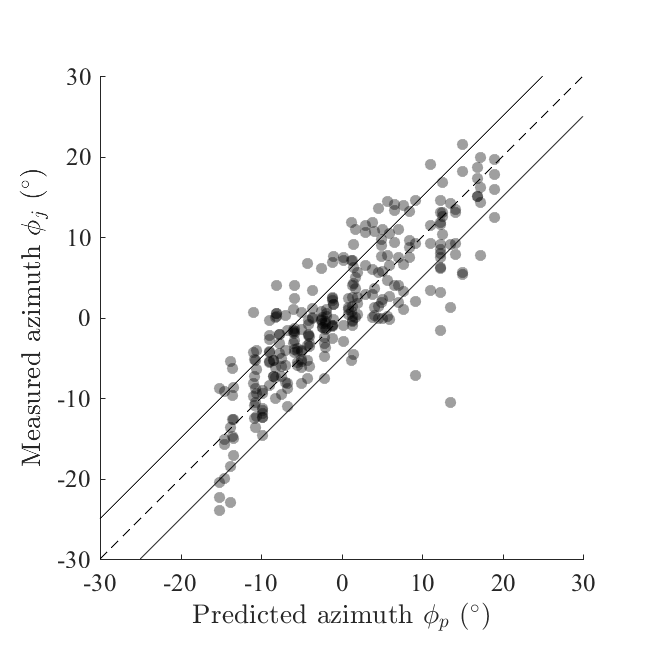
\includegraphics[width=\textwidth]{05_proposed_models/figures/LocalizationModelResults}
        \caption{Proposed model}
        \label{fig:Localization_Model_Results}
  \end{subfigure}
  \hfill
  \begin{subfigure}[b]{0.49\columnwidth}
        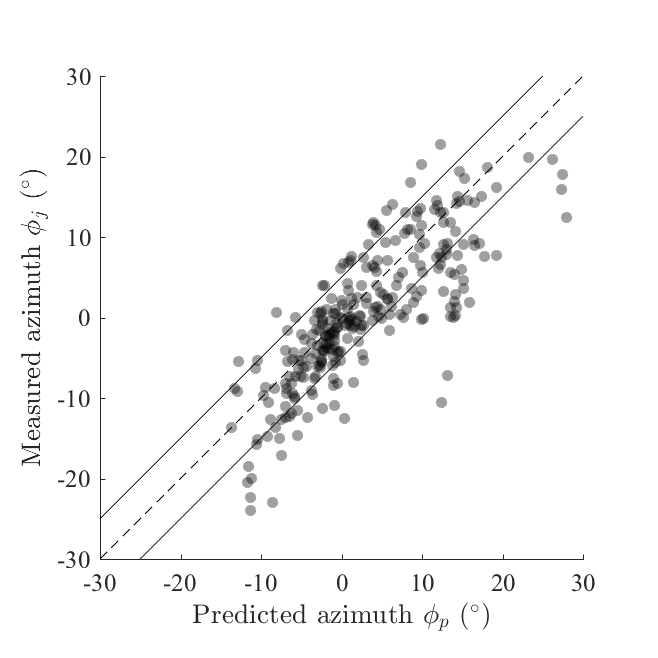
\includegraphics[width=\textwidth]{05_proposed_models/figures/DietzLocalizationResults}
        \caption{\citet{Dietz2011} model}
        \label{fig:Dietz_Localization_Results}
  \end{subfigure}
  \caption[Scatter plots of measured versus predicted source directions.]{
  Scatter plots of measured versus predicted source directions.
  The transparent filled circles indicate the data and model values;
  the dashed lines indicate ideal model results (i.e., $\phi_j = \phi_p$);
  the solid lines indicate discrepancies of $5^\circ$ (i.e., $\phi_j = \phi_p \pm 5^\circ$).}
  \label{fig:Localization_Model_Comparison}
\end{figure}

For both models we observe two outlying data points at approximately $(\phi_p, \phi_j) = (+10^\circ, -10^\circ)$, for which the predicted directions are to the listener's left ($+$), while that subject (both of these data points are from the same subject) localized the sound to the right ($-$).
Although not shown here, the same data points appear again as outliers when plotted against the \textit{intended} source direction, suggesting that these outliers could well be due to an error on the part of the subject.

%% Coloration results
\subsection{Comparison of coloration models}\label{sec:05_Proposed_Models:Coloration_Results}
Using the MUSHRA ratings collected from the coloration listening test (described in \secref{sec:05_Proposed_Models:Coloration_Test}), we performed linear regressions for each model listed in \secref{sec:05_Proposed_Models:Coloration_Models}.
We first converted the MUSHRA ratings to ``coloration scores'', given by $C = 100 - M$, where $M$ are the MUSHRA ratings.
Through this transformation, a reference sample will always have a coloration score of zero, while the low-pass anchor will have a coloration score of 100.
We then computed linear regressions between the values of the metrics in each of the four models and the coloration scores.
Note that, for the binaural models (\citet{Pulkki1999} and \citet{Wittek2007}), we computed each metric on a per-subject basis, i.e., using each subject's individualized HRTFs to render to binaural and subsequently computing per-subject values of each metric.

In building the coloration models, an analysis of the statistical significance of each model parameter revealed that, for the proposed model, neither $\sigma_\eta$ nor $E_{\text{pk}}$ provided a significant improvement to the model.
This is likely because, for all of our test samples, both $\sigma_\eta$ and $E_{\text{pk}}$ were strongly correlated with $\rho_\eta$.
Consequently, our proposed model uses only $\rho_\eta$ and $E_\text{n}$.
Additionally, a ``$y$-intercept'' (offset) term was considered for each model, but was found to be statistically insignificant in all cases.%
\footnote{This is likely because all of the reference samples, by definition, obtain zero coloration scores and zero values for each metric.}
The final formulae and corresponding Pearson correlation coefficients between the measured and predicted coloration scores are tabulated in \tabref{tab:Coloration_Model_Formulas}.
These correlation coefficients suggest that the proposed model is best able to predict the measured coloration scores.

The proposed model is also the only model to have both coefficients positive, even though all of the metrics listed in \secref{sec:04_Auditory_Models:Coloration_Metrics} produce positive values for non-flat spectra.
This indicates that both metrics in the proposed model directly contribute to perceived coloration.
We also note the similarity between the two binaural models (\citet{Pulkki1999} and \citet{Wittek2007}), in both the coefficients and performance of the model.
This may be explained by both models capturing essentially the same information through combining the binaural spectra (see \secreftwo{sec:04_Auditory_Models:Coloration_Metrics:Pulkki_CLL}{sec:04_Auditory_Models:Coloration_Metrics:Wittek_IS}).

\begin{table}[t]
\centering
 \begin{tabular}{|c|c|c|} \hline
 \textbf{Model Name} & \textbf{Formula} & \textbf{Correlation} \\ \hline
 Proposed & $C = 2.88 \rho_\eta + 1.74 E_\text{n}$ & 0.84 \\
 \citet{Kates1984} & $C = -3.20 \rho_{e_\text{CS}} + 54.16 \sigma_{e_\text{CS}}$ & 0.72 \\
 \citet{Pulkki1999} & $C = 9.84 \rho_{e_\text{CLL}} - 18.38 \sigma_{e_\text{CLL}}$ & 0.77 \\
 \citet{Wittek2007} & $C = 10.35 \rho_{e_\text{IS}} - 19.58 \sigma_{e_\text{IS}}$ & 0.77 \\ \hline
 \end{tabular}
 \caption[Formulae and correlation coefficients for each coloration model.]{
 Formulae and Pearson correlation coefficients for each coloration model.
 All correlation $p$-values were less than $10^{-17}$.}
 \label{tab:Coloration_Model_Formulas}
\end{table}

Additionally, in \figref{fig:Coloration_Model_Comparison}, the measured coloration scores are plotted against the predicted scores for each model.
From these plots, we see that the proposed model produces the most compact (towards the $y = x$ line) distribution of the data.
We also note that the model of \citet{Kates1984} is the only model that consistently under-predicts the low anchor scores (as indicated by the cluster of data points at approximately $(75,100)$ in the second plot).
This suggests that this model did not have sufficient degrees of freedom (since the two metrics were strongly correlated with one another) to both capture the end points of the data and fit the intermediate points.

\begin{figure}[t]
\centering
  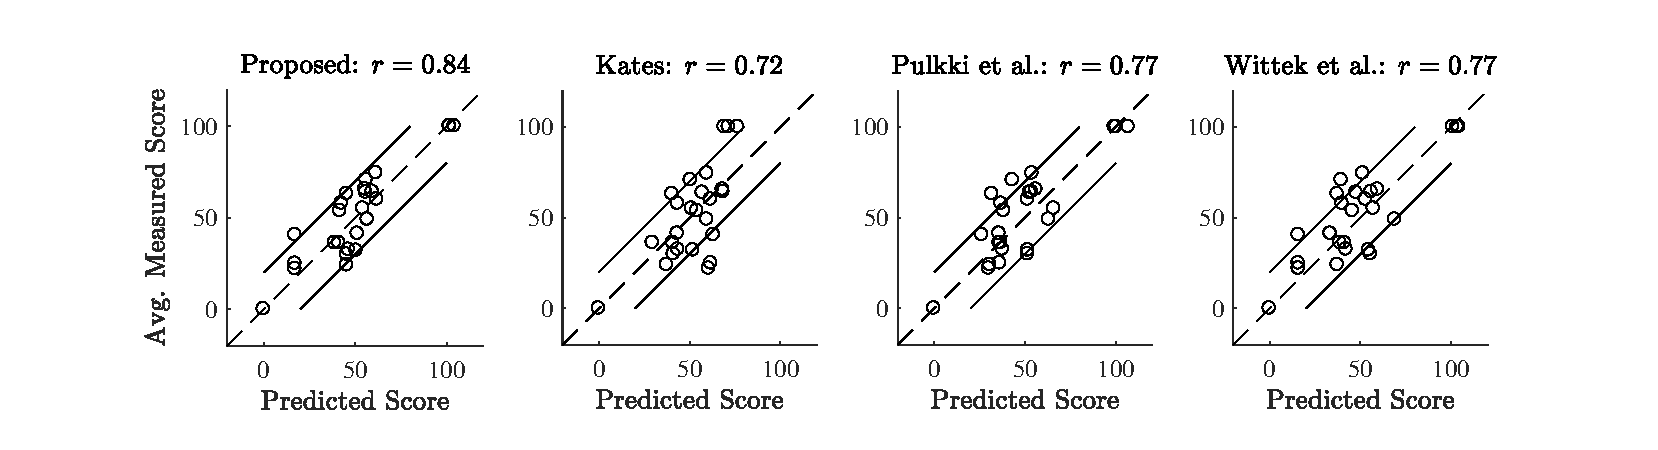
\includegraphics[width=0.99\textwidth,trim={2.15cm 0.3cm 2.3cm 0.5cm},clip]{05_proposed_models/figures/ColorationModelComparison}
  \caption[Scatter plots of average measured versus predicted coloration scores.]{
  Scatter plots of average measured versus predicted coloration scores for each model.
  The empty circles indicate the data and model values;
  the dashed lines indicate ideal model results (i.e., $y = x$);
  the solid lines indicate discrepancies of 20 points (i.e., $y = x \pm 20$).
  The predicted coloration scores for the binaural models (\citet{Pulkki1999} and \citet{Wittek2007}) are averaged across listeners.
  Correlation coefficients for each set of data are given at the top of each plot.}
  \label{fig:Coloration_Model_Comparison}
\end{figure}

\begin{figure}[t]
  \centering
  \setlength{\fboxsep}{0pt}
  \setlength{\fboxrule}{1pt}
  \fbox{\includegraphics[page=1,width=0.99\textwidth]{05_proposed_models/figures/test_instructions}}
  \caption{Instructions provided to each subject for the localization test.}
  \label{fig:05_Proposed_Models:Localization_Instructions}
\end{figure}

\begin{figure}[t]
  \centering
  \setlength{\fboxsep}{0pt}
  \setlength{\fboxrule}{1pt}
  \fbox{\includegraphics[page=2,width=0.99\textwidth]{05_proposed_models/figures/test_instructions}}
  \caption{Instructions provided to each subject for the coloration test.}
  \label{fig:05_Proposed_Models:Coloration_Instructions}
\end{figure}

\section{Conclusions}\label{sec:05_Proposed_Models:Conclusions}
In this work, we developed models for perceived source localization and spectral coloration.
We empirically determined values for the parameters of these models through comparison with results of subjective listening experiments that we conducted.
The primary advantage of these models, compared to existing binaural ones, is that they do not require rendering ambisonics to binaural.
This allows the models to be used to directly evaluate navigational methods for ambisonics-encoded sound fields, without introducing extraneous factors such as the choice of ambisonics-to-binaural rendering approach or of HRTF.%
\footnote{While it is our expectation that such extraneous factors will necessarily conflate their corresponding errors with those introduced by the navigational method under test, it is worth noting that the relative magnitudes of such errors have not been established.
This remains a topic for further study.}

The localization model (described in \secref{sec:05_Proposed_Models:Localization_Model}) extends a recently-developed precedence-effect-based energy vector model \citep{Stitt2016} in order to predict perceived source localization directly from the ambisonics impulse responses.
To determine parameters of the model, we conducted a virtual localization test (described in \secref{sec:05_Proposed_Models:Localization_Test}) with individualized binaural rendering over head-tracked and equalized headphones.
The predictions of the localization model (see \secref{sec:05_Proposed_Models:Localization_Results}) are in good agreement with the results of this localization test, achieving a mean absolute prediction error of $3.67^\circ$.
Furthermore, the proposed model performs comparably to, if not better than, the binaural localization model of \citet{Dietz2011} (described in \secref{sec:04_Auditory_Models:Binaural_Localization_Model}), in terms of its agreement with the data.

Two important caveats to this result are 1) that the model requires experimental data in order to determine values for its free parameters and 2) that these values are not necessarily valid over any conditions other than those tested.
Indeed, it is worth emphasizing that this model has only been validated for frontal ($\pm20^\circ$ azimuth) sources and a speech signal.
However, given the accuracy of the predictions yielded by the model and the relatively small number of degrees of freedom compared to the number of data points, we conclude that the \textit{structure} of the model is generally valid.
Therefore, we take the parameter values determined here to define a default specification of the model, which we can expect to provide \textit{plausible} predictions of source localization, even though the accuracy of those predictions will almost certainly degrade for any conditions other than those tested here.
The magnitudes of such degradations under other conditions (e.g., source positions, navigational methods, stimuli, etc.) remain to be determined.

Future refinements to this model might pursue reducing its number of free parameters by developing (possibly empirical) models for those parameters based on some input data.
For example, one might seek a model for the stimulus-dependent stationary signal weight ($\alpha$), which is currently determined empirically by fitting model predictions to experimental data (see \citet{Stitt2016,Stitt2017}), such that it can be determined \textit{a priori} for a given stimulus.%
\footnote{\citet{Stitt2016} suggest a simple model for $\alpha$ based on interaural time differences of leading and lagging signals, but no direct relationship between the stimulus and $\alpha$ is given.}

The coloration model uses only the omnidirectional ambisonics impulse responses (i.e., the free-field transfer functions) and predicts a perceived ``coloration score'' from a linear combination of two metrics (defined in \secref{sec:04_Auditory_Models:Coloration_Metrics}): the range of the auditory band spectral error ($\rho_\eta$) and the notch errors ($E_\text{n}$).
To construct this model, we conducted a MUSHRA \citep{ITU-R-BS.1534-3} test (described in \secref{sec:05_Proposed_Models:Coloration_Test}) and performed a linear regression of the metrics with the collected subjective ratings of coloration.
We compared the proposed model to several alternative models and found it to achieve the highest correlation to the measured data (see \secref{sec:05_Proposed_Models:Coloration_Results}).

As with the localization model, the validity of the proposed coloration model has only been established for a limited set of conditions.
Additionally, predicting these ``coloration scores'' is a somewhat artificial task, as the scale (0--100) is arbitrary, and there is no reason to think that the perceived coloration should be strictly linearly related to any of the metrics used.
Nevertheless, a more general result of this analysis is that the metrics used in the proposed model ($\rho_\eta$ and $E_\text{n}$) are dominant factors in the perception of coloration.
Thus, each of these metrics may serve as a useful measure of perceptible spectral coloration, as a large value for either metric would almost certainly entail perceptible coloration.

Ultimately, in order to more rigorously establish their psychoacoustic relevance, the auditory models proposed here should be further validated through additional listening experiments with more subjects and spanning a wider range of conditions.
%The coloration model in particular should be validated for a larger set of navigational methods, since the spectral colorations considered in this work may or may not be comparable to those induced by alternative methods.
Despite this eventual need for further validation, we expect that these models will nonetheless yield valuable insights when evaluating navigational methods.
Consequently, comprehensive comparisons of existing navigational methods should be conducted using these models in order to quantify the penalties incurred by each method, and ultimately determine limits of usability for each method (e.g., maximum translation distance with $\leq 5^\circ$ source localization error).
Indeed, throughout the rest of the present thesis, we employ both the proposed localization model to predict localization and the spectral error metric, $\rho_\eta$, as a measure of perceived coloration.

\section*{Acknowledgements}
The ambisonics room impulse responses were recorded using the Eigenmike by mh Acoustics \citep{EigenmikeURL}.
The present author wishes to thank P.~Stitt for providing the MATLAB code for the precedence-effect-based energy vector model (available online).\citefooturl{StittCodeURL}
This work was approved by the Institutional Review Board for human subjects research at Princeton University,
and was originally presented by \citeauthor{TylkaChoueiri2017a} at the 173\textsuperscript{rd} Meeting of Acoustical Society of America (Acoustics '17 Boston) and published in \textit{Proceedings of Meetings on Acoustics} \citep{TylkaChoueiri2017a}.